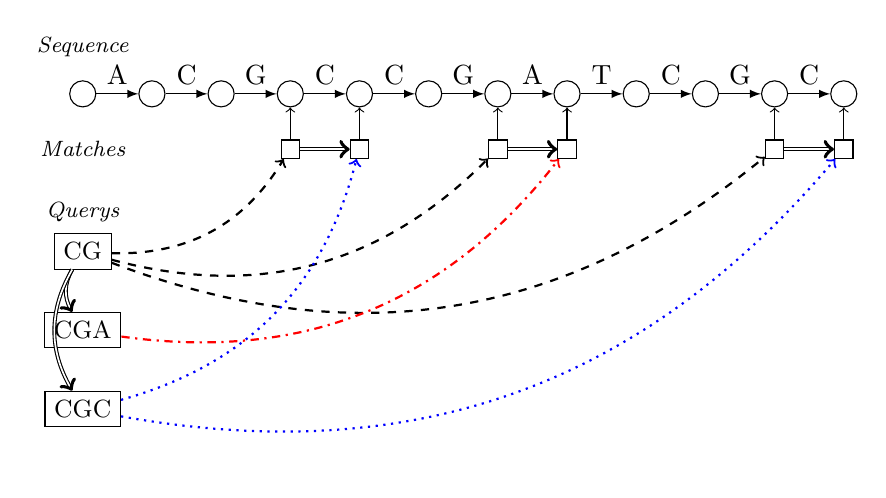
\begin{tikzpicture}[auto]
	\tikzstyle{state} = [ draw, circle, thin, node distance = 2.5em, font={\small}];
	\tikzstyle{query} = [ draw, rectangle, thin, node distance = 2.5em, font={\small}];
	\tikzstyle{info} = [font={\itshape\footnotesize}]
	\tikzstyle{point}  = [ ->, thin, font={\small}];
	\tikzstyle{extend} = [ ->, double, font={\small}];
	\tikzstyle{trace} = [ ->, thick, dashed, bend right, font={\small} ];

	\def \seq {X,A,C,G,C,C,G,A,T,C,G,C}

	\foreach \x [count=\xi] in \seq {
		\ifnum 1 < \xi
			\pgfmathparse{int(\xi-1)}
			\let \li \pgfmathresult
			\node[state, right of=\li] (\xi) {};
			\draw[->, >=latex] (\li) to node{\x} (\xi);
		\else
			\node[state] (\xi) {};
		\fi
	}

	\node[info] at (0,0.6) {Sequence};
	\node[info] at (0,-0.7) {Matches};
	\node[info] at (0,-1.5) {Querys};

	\node[query](CG)  at (0,-2) {CG};
	\node[query](CGA) at (0,-3) {CGA};
	\node[query](CGC) at (0,-4) {CGC};

	\tikzstyle{traceCG} = [ ->, thick, dashed, bend right, color=black ];
	\tikzstyle{traceCGA} = [ ->, thick, dashdotted, bend right, color=red ];
	\tikzstyle{traceCGC} = [ ->, thick, dotted, bend right, color=blue ];

	\draw[extend, bend right] (CG) to (CGA);
	\draw[extend, bend right] (CG) to (CGC);

	\foreach \xi/\xv in {4/CG,7/CG,11/CG} {
		\node[draw, below of=\xi, node distance=2em] (p\xi) {};
		\draw[point] (p\xi) to (\xi);
		\draw[trace\xv] (\xv) to (p\xi);
	}

	\foreach \xi/\xv in {5/CGC,8/CGA,12/CGC} {
		\node[draw, below of=\xi, node distance=2em] (p\xi) {};
		\draw[point] (p\xi) to (\xi);
		\draw[trace\xv] (\xv) to (p\xi);
	}

	\foreach \xi/\yi in {4/5,7/8,11/12} {
		\draw[extend] (p\xi) to (p\yi);
	}
\end{tikzpicture}
